% GNUPLOT: LaTeX picture with Postscript
\documentclass{minimal}
% Set font size
\makeatletter
\def\@ptsize{1}
\InputIfFileExists{size11.clo}{}{%
   \GenericError{(gnuplot) \space\space\space\@spaces}{%
      Gnuplot Error: File `size11.clo' not found! Could not set font size%
   }{See the gnuplot documentation for explanation.%
   }{For using a font size a file `size<fontsize>.clo' has to exist.
        Falling back ^^Jto default fontsize 10pt.}%
  \def\@ptsize{0}
  \input{size10.clo}%
}%
\makeatother
% Load packages
\usepackage{calc}
\usepackage{graphicx}
\usepackage{color}
\makeatletter
% Select an appropriate default driver (from TeXLive graphics.cfg)
\begingroup
  \chardef\x=0 %
  % check pdfTeX
  \@ifundefined{pdfoutput}{}{%
    \ifcase\pdfoutput
    \else
      \chardef\x=1 %
    \fi
  }%
  % check VTeX
  \@ifundefined{OpMode}{}{%
    \chardef\x=2 %
  }%
\expandafter\endgroup
\ifcase\x
  % default case
  \PassOptionsToPackage{dvips}{geometry}
\or
  % pdfTeX is running in pdf mode
  \PassOptionsToPackage{pdftex}{geometry}
\else
  % VTeX is running
  \PassOptionsToPackage{vtex}{geometry}
\fi
\makeatother
% Set papersize
\usepackage[papersize={576.00bp,432.00bp},text={576.00bp,432.00bp}]{geometry}
% No page numbers and no paragraph indentation
\pagestyle{empty}
\setlength{\parindent}{0bp}%
% Load configuration file
\InputIfFileExists{gnuplot.cfg}{%
  \typeout{Using configuration file gnuplot.cfg}%
}{%
 \typeout{No configuration file gnuplot.cfg found.}%
}%
%
\begin{document}
\begingroup
  \makeatletter
  \providecommand\color[2][]{%
    \GenericError{(gnuplot) \space\space\space\@spaces}{%
      Package color not loaded in conjunction with
      terminal option `colourtext'%
    }{See the gnuplot documentation for explanation.%
    }{Either use 'blacktext' in gnuplot or load the package
      color.sty in LaTeX.}%
    \renewcommand\color[2][]{}%
  }%
  \providecommand\includegraphics[2][]{%
    \GenericError{(gnuplot) \space\space\space\@spaces}{%
      Package graphicx or graphics not loaded%
    }{See the gnuplot documentation for explanation.%
    }{The gnuplot epslatex terminal needs graphicx.sty or graphics.sty.}%
    \renewcommand\includegraphics[2][]{}%
  }%
  \providecommand\rotatebox[2]{#2}%
  \@ifundefined{ifGPcolor}{%
    \newif\ifGPcolor
    \GPcolortrue
  }{}%
  \@ifundefined{ifGPblacktext}{%
    \newif\ifGPblacktext
    \GPblacktexttrue
  }{}%
  % define a \g@addto@macro without @ in the name:
  \let\gplgaddtomacro\g@addto@macro
  % define empty templates for all commands taking text:
  \gdef\gplbacktext{}%
  \gdef\gplfronttext{}%
  \makeatother
  \ifGPblacktext
    % no textcolor at all
    \def\colorrgb#1{}%
    \def\colorgray#1{}%
  \else
    % gray or color?
    \ifGPcolor
      \def\colorrgb#1{\color[rgb]{#1}}%
      \def\colorgray#1{\color[gray]{#1}}%
      \expandafter\def\csname LTw\endcsname{\color{white}}%
      \expandafter\def\csname LTb\endcsname{\color{black}}%
      \expandafter\def\csname LTa\endcsname{\color{black}}%
      \expandafter\def\csname LT0\endcsname{\color[rgb]{1,0,0}}%
      \expandafter\def\csname LT1\endcsname{\color[rgb]{0,1,0}}%
      \expandafter\def\csname LT2\endcsname{\color[rgb]{0,0,1}}%
      \expandafter\def\csname LT3\endcsname{\color[rgb]{1,0,1}}%
      \expandafter\def\csname LT4\endcsname{\color[rgb]{0,1,1}}%
      \expandafter\def\csname LT5\endcsname{\color[rgb]{1,1,0}}%
      \expandafter\def\csname LT6\endcsname{\color[rgb]{0,0,0}}%
      \expandafter\def\csname LT7\endcsname{\color[rgb]{1,0.3,0}}%
      \expandafter\def\csname LT8\endcsname{\color[rgb]{0.5,0.5,0.5}}%
    \else
      % gray
      \def\colorrgb#1{\color{black}}%
      \def\colorgray#1{\color[gray]{#1}}%
      \expandafter\def\csname LTw\endcsname{\color{white}}%
      \expandafter\def\csname LTb\endcsname{\color{black}}%
      \expandafter\def\csname LTa\endcsname{\color{black}}%
      \expandafter\def\csname LT0\endcsname{\color{black}}%
      \expandafter\def\csname LT1\endcsname{\color{black}}%
      \expandafter\def\csname LT2\endcsname{\color{black}}%
      \expandafter\def\csname LT3\endcsname{\color{black}}%
      \expandafter\def\csname LT4\endcsname{\color{black}}%
      \expandafter\def\csname LT5\endcsname{\color{black}}%
      \expandafter\def\csname LT6\endcsname{\color{black}}%
      \expandafter\def\csname LT7\endcsname{\color{black}}%
      \expandafter\def\csname LT8\endcsname{\color{black}}%
    \fi
  \fi
    \setlength{\unitlength}{0.0500bp}%
    \ifx\gptboxheight\undefined%
      \newlength{\gptboxheight}%
      \newlength{\gptboxwidth}%
      \newsavebox{\gptboxtext}%
    \fi%
    \setlength{\fboxrule}{0.5pt}%
    \setlength{\fboxsep}{1pt}%
    \definecolor{tbcol}{rgb}{1,1,1}%
\begin{picture}(11520.00,8640.00)%
    \gplgaddtomacro\gplbacktext{%
      \csname LTb\endcsname%%
      \put(1188,4970){\makebox(0,0)[r]{\strut{}\Large$0.1$}}%
      \put(1188,5900){\makebox(0,0)[r]{\strut{}\Large$1$}}%
      \put(1188,6829){\makebox(0,0)[r]{\strut{}\Large$10$}}%
      \put(1188,7759){\makebox(0,0)[r]{\strut{}\Large$100$}}%
      \put(2319,4100){\makebox(0,0){\strut{}}}%
      \put(5637,4100){\makebox(0,0){\strut{}}}%
      \put(5459,7759){\makebox(0,0)[l]{\strut{}\huge(a)}}%
      \put(7184,7346){\makebox(0,0)[l]{\strut{}\large$N^{0.8}$}}%
      \put(7184,6865){\makebox(0,0)[l]{\strut{}\large$N^{0.6}$}}%
      \put(7184,6383){\makebox(0,0)[l]{\strut{}\large$N^{0.4}$}}%
      \put(7184,5971){\makebox(0,0)[l]{\strut{}\large$N^{0.2}$}}%
      \put(7184,5059){\makebox(0,0)[l]{\strut{}\large$N^{0}$}}%
    }%
    \gplgaddtomacro\gplfronttext{%
      \csname LTb\endcsname%%
      \put(9161,7731){\makebox(0,0)[r]{\strut{}\Large$\alpha=1.1$}}%
      \csname LTb\endcsname%%
      \put(9161,7331){\makebox(0,0)[r]{\strut{}\Large$\alpha=1.2$}}%
      \csname LTb\endcsname%%
      \put(9161,6931){\makebox(0,0)[r]{\strut{}\Large$\alpha=1.3$}}%
      \csname LTb\endcsname%%
      \put(9161,6531){\makebox(0,0)[r]{\strut{}\Large$\alpha=1.4$}}%
      \csname LTb\endcsname%%
      \put(9161,6131){\makebox(0,0)[r]{\strut{}\Large$\alpha=1.5$}}%
      \csname LTb\endcsname%%
      \put(9161,5731){\makebox(0,0)[r]{\strut{}\Large$\alpha=1.6$}}%
      \csname LTb\endcsname%%
      \put(9161,5331){\makebox(0,0)[r]{\strut{}\Large$\alpha=1.8$}}%
      \csname LTb\endcsname%%
      \put(9161,4931){\makebox(0,0)[r]{\strut{}\Large$\alpha=2.0$}}%
      \csname LTb\endcsname%%
      \put(583,6039){\rotatebox{-270.00}{\makebox(0,0){\strut{}\huge$\kappa_N$}}}%
    }%
    \gplgaddtomacro\gplbacktext{%
      \csname LTb\endcsname%%
      \put(1596,6888){\makebox(0,0)[r]{\strut{}$0$}}%
      \put(1596,7384){\makebox(0,0)[r]{\strut{}$1$}}%
      \put(1596,7879){\makebox(0,0)[r]{\strut{}$2$}}%
      \put(1596,8375){\makebox(0,0)[r]{\strut{}$3$}}%
      \put(1728,6519){\makebox(0,0){\strut{}0}}%
      \put(2942,6519){\makebox(0,0){\strut{}10}}%
      \put(4156,6519){\makebox(0,0){\strut{}20}}%
    }%
    \gplgaddtomacro\gplfronttext{%
      \csname LTb\endcsname%%
      \put(4340,8046){\makebox(0,0)[r]{\strut{}\Large$\displaystyle\int^t_0 ds C_N(s)$}}%
      \csname LTb\endcsname%%
      \put(4340,7646){\makebox(0,0)[r]{\strut{}\Large$C_N(t)$}}%
      \csname LTb\endcsname%%
      \put(4895,6739){\makebox(0,0){\strut{}\Large$t$}}%
      \put(2717,7263){\makebox(0,0){\strut{}\Large$\alpha=1.3$}}%
    }%
    \gplgaddtomacro\gplbacktext{%
      \csname LTb\endcsname%%
      \put(1188,1272){\makebox(0,0)[r]{\strut{}\Large$0.1$}}%
      \put(1188,2444){\makebox(0,0)[r]{\strut{}\Large$1$}}%
      \put(1188,3615){\makebox(0,0)[r]{\strut{}\Large$10$}}%
      \put(2319,440){\makebox(0,0){\strut{}\Large100}}%
      \put(5637,440){\makebox(0,0){\strut{}\Large1000}}%
      \put(5459,3954){\makebox(0,0)[l]{\strut{}\huge(b)}}%
      \put(7184,4027){\makebox(0,0)[l]{\strut{}\large$N^{0.8}$}}%
      \put(7184,3368){\makebox(0,0)[l]{\strut{}\large$N^{0.6}$}}%
      \put(7184,2783){\makebox(0,0)[l]{\strut{}\large$N^{0.4}$}}%
      \put(7184,2270){\makebox(0,0)[l]{\strut{}\large$N^{0.2}$}}%
      \put(7184,1374){\makebox(0,0)[l]{\strut{}\large$N^{0}$}}%
    }%
    \gplgaddtomacro\gplfronttext{%
      \csname LTb\endcsname%%
      \put(9161,4120){\makebox(0,0)[r]{\strut{}\Large$\alpha=1.1$}}%
      \csname LTb\endcsname%%
      \put(9161,3720){\makebox(0,0)[r]{\strut{}\Large$\alpha=1.2$}}%
      \csname LTb\endcsname%%
      \put(9161,3320){\makebox(0,0)[r]{\strut{}\Large$\alpha=1.3$}}%
      \csname LTb\endcsname%%
      \put(9161,2920){\makebox(0,0)[r]{\strut{}\Large$\alpha=1.4$}}%
      \csname LTb\endcsname%%
      \put(9161,2520){\makebox(0,0)[r]{\strut{}\Large$\alpha=1.5$}}%
      \csname LTb\endcsname%%
      \put(9161,2120){\makebox(0,0)[r]{\strut{}\Large$\alpha=1.6$}}%
      \csname LTb\endcsname%%
      \put(9161,1720){\makebox(0,0)[r]{\strut{}\Large$\alpha=1.8$}}%
      \csname LTb\endcsname%%
      \put(9161,1320){\makebox(0,0)[r]{\strut{}\Large$\alpha=2.0$}}%
      \csname LTb\endcsname%%
      \put(583,2490){\rotatebox{-270.00}{\makebox(0,0){\strut{}\huge$C_N(0)$}}}%
      \put(4769,330){\makebox(0,0){\strut{}\huge$N$}}%
    }%
    \gplbacktext
    \put(0,0){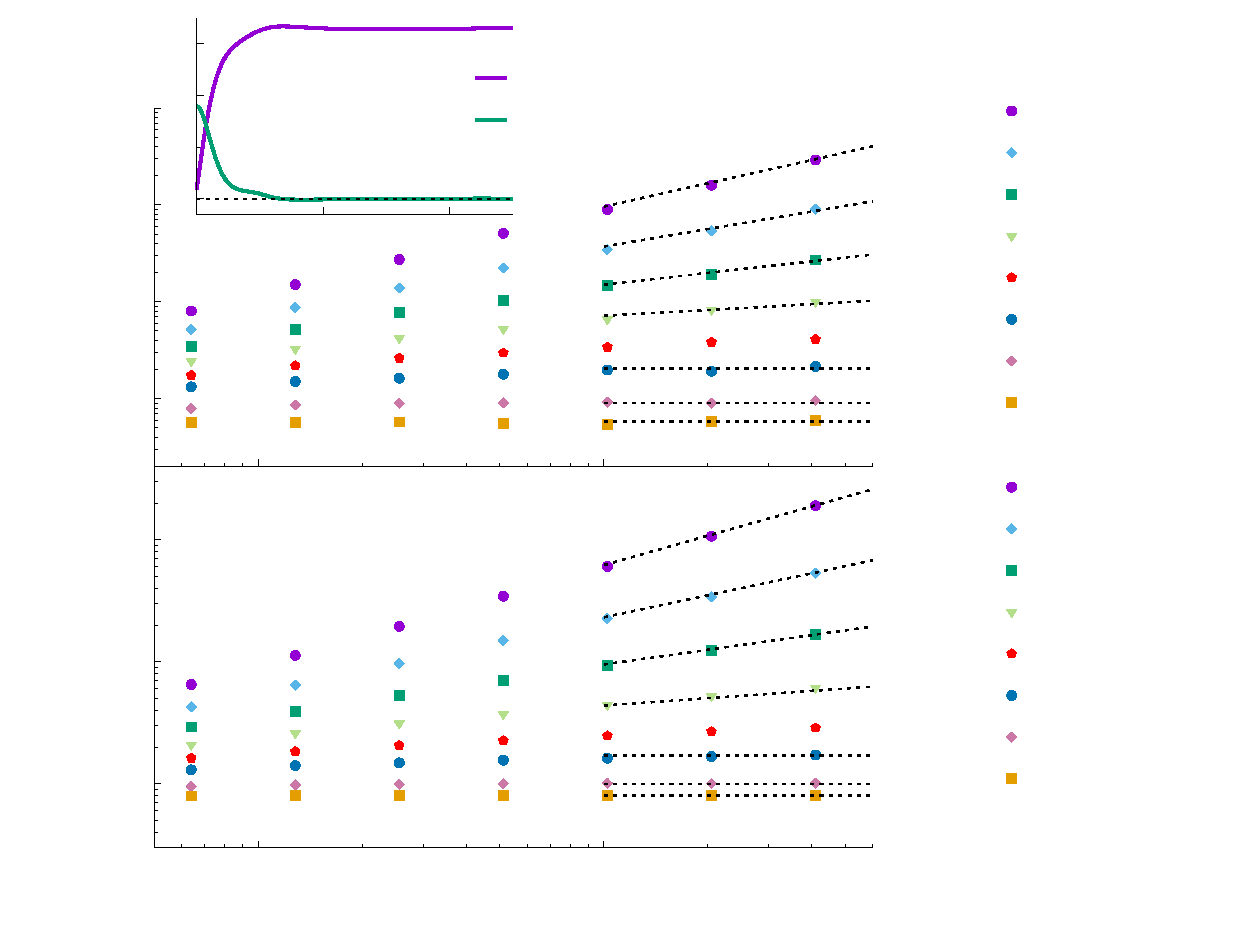
\includegraphics[width={576.00bp},height={432.00bp}]{fig1-inc}}%
    \gplfronttext
  \end{picture}%
\endgroup
\end{document}
